\documentclass[11pt,fleqn]{article}

\setlength {\topmargin} {-.15in}
\setlength {\textheight} {8.6in}

\usepackage{amsmath}
\usepackage{amssymb}
\usepackage{color}
\usepackage{tikz}
\usetikzlibrary{automata,positioning,arrows}
\usepackage{diagbox}
\usepackage{stackrel}

\newcommand{\be}{\begin{enumerate}}
\newcommand{\ee}{\end{enumerate}}

\begin{document}
\textbf{Exercise 4.1.32:} Parallel edge detection. Devise a linear-time algorithm to count the parallel
edges in a graph.\\

\textbf{Solution:}
\begin{itemize}
	\item Keep track of all the vertices adjacent to a vertex using a HashSet,array or any data structure of your choice. This is basically the idea of an adjacency list for each vertex.
	
	\item Iterate through all vertices in the graph and mark the adjacent vertices if not yet seen in the set or array of visited nodes.
	
	\item If vertex has been seen, that means it is a parallel edge. Increment the counter.
	
	\item Once all edges accounted for, divide the edgecounter by 2 to remove seeing duplicate edges
\end{itemize}

Pseudocode below:

\begin{center}
	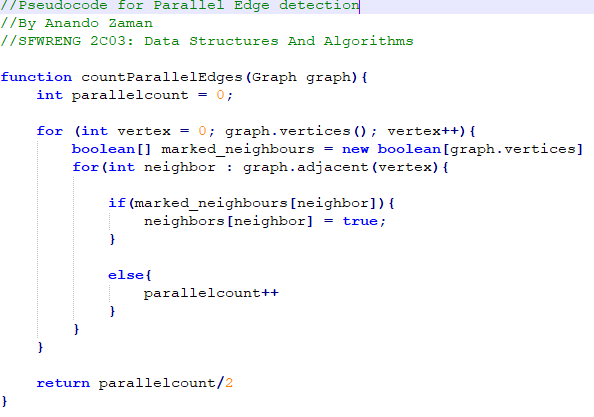
\includegraphics[scale=1]{4.1.32.png}
\end{center}


\end{document}
